\section{模型检验与误差分析}

验证围绕输入处理、方程口径、数值离散、独立实现和结构情景展开。题目未提供药材内部温湿实测值、参数分布或重复实验，因此本节评价数值一致性，并将物理预测能力单独讨论。

\subsection{边界、量纲与极端情景检查}

式\eqref{eq:heat-fixed}两侧单位均为$\mathrm{W/m^3}$，式\eqref{eq:moist-fixed}两侧均为$\mathrm{s^{-1}}$；表面热通量和水分归一化通量分别为$\mathrm{W/m^2}$与$\mathrm{m/s}$。问题四中$D/R^2$具有$\mathrm{s^{-1}}$量纲，材料坐标变换前后保持一致。

程序通过五项极端测试：常场绝热时右端为零；关闭扩散和传质后，非均匀干基含水率随材料收缩保持不变；令$R(t)$为常数时，问题四退化为固定域离散式；计算到72 h即停止调用半径插值；人造非中心湿峰可被全域事件识别。这些结果用于检查符号、坐标和判停逻辑。

\subsection{网格、时间步、守恒与独立求解}

表\ref{tab:verification-summary}汇总主解与独立P1有限元的公共点差异。独立程序使用一致质量矩阵、Gauss积分、节点Robin边界和自编BDF2，不调用主有限体积程序的面通量、表面恢复或事件函数。问题一热场另与512项Fourier--Bessel解析级数比较，全时域最大差为$1.285\times10^{-6}\ ^\circ\mathrm C$。

\begin{table}[htbp]
  \caption{独立求解对照}
  \label{tab:verification-summary}
  \centering
  \begin{tabular}{lrrl}
    \toprule
    对象 & 最大温差/$^\circ$C & 最大含水率差 & 抽检范围 \\
    \midrule
    问题一 & $1.801\times10^{-6}$ & $1.321\times10^{-6}$ & 10个稠密剖面 \\
    问题二 & $9.161\times10^{-6}$ & $3.222\times10^{-6}$ & 6个题定时刻 \\
    问题三 & $3.028\times10^{-5}$ & $3.308\times10^{-7}$ & 108个保存时刻 \\
    问题四 & $1.093\times10^{-5}$ & $6.030\times10^{-6}$ & 110个公共时刻 \\
    \bottomrule
  \end{tabular}
\end{table}

固定域的归一化水分累计残差为
\begin{equation}
E_C=\bar C-C_0+\int_0^t\frac{2h_m}{R_0}(C_s-C_{\mathrm{eq}})\,\mathrm d\tau.
\end{equation}
当$b(C)$变化时，以$H=\overline{b(C)(T-T_0)}$构造的有效热收支还需包含$b'(C)(T-T_0)C_t$修正项。四问水分与修正热学收支的最大归一化残差均小于$1.1\times10^{-9}$，表明离散轨迹与所建方程一致。潜热等未建模项的影响列入模型局限。

图\ref{fig:numerical-validation}(a)--(c)显示相邻网格差总体呈近二阶下降；(d)把最大步长、容差与Radau积分器的终点差异放到同一对数尺度；(e)(f)分别给出独立有限元和累计守恒两条异源证据。问题三、四的1280与2560网格临界时间差分别为$0.07596$ s和$0.05797$ s；时间步上限30 s减半后的变化为$0.000755$ s和$0.000462$ s。按近二阶关系估计，主网格终点的数值尺度约为$0.1013$ s和$0.0773$ s，本文据此采用$0.1$ s量级作为保守表述。

\begin{figure}[htbp]
  \centering
  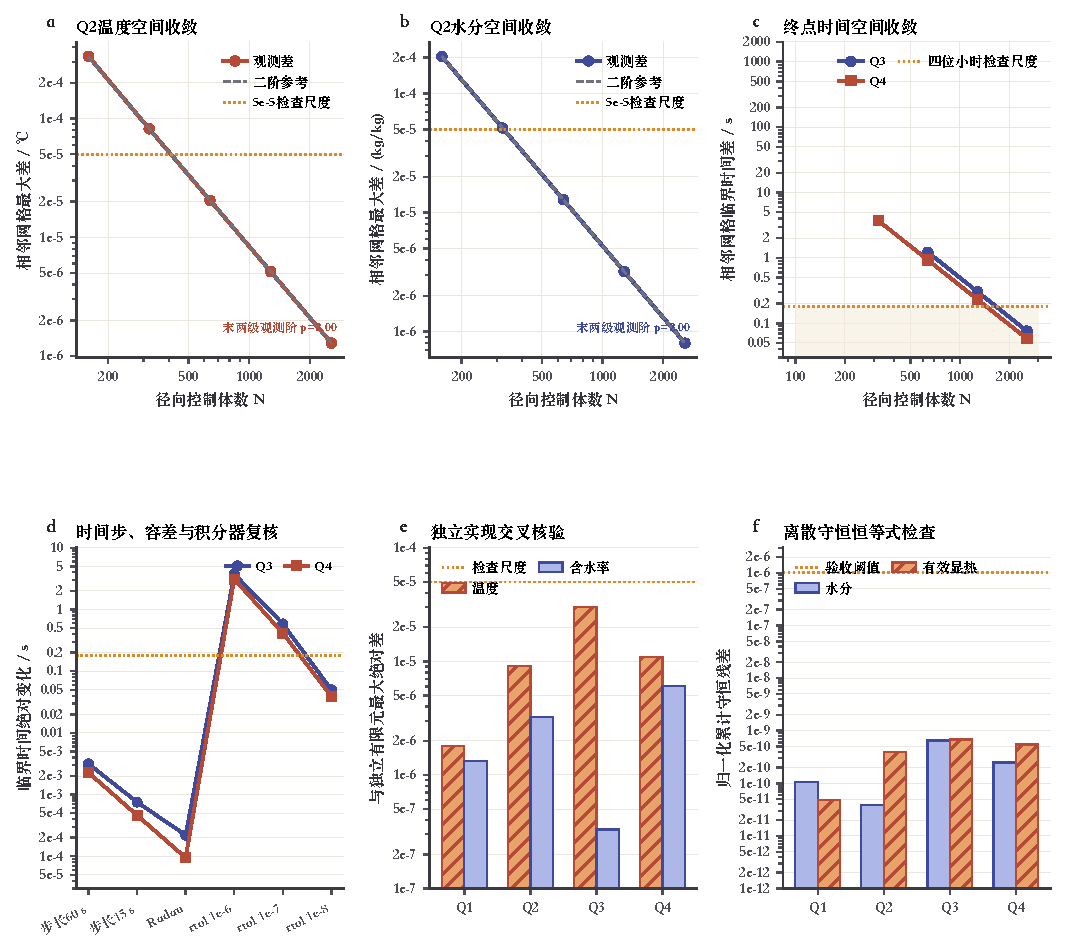
\includegraphics[width=\textwidth]{figures/fig06_numerical_validation.pdf}
  \caption{数值收敛与独立验证}
  \label{fig:numerical-validation}
\end{figure}

临界附近$g(t)$的斜率分别约为
\[
-2.913\times10^{-7}\quad\text{和}\quad
-5.135\times10^{-7}\ \mathrm{(kg/kg)/s}.
\]
由$\delta t\approx\delta C/|g'|$可知，含水率显示误差$5\times10^{-5}$可对应问题三约172 s、问题四约97 s的时间尺度。因此，表格小数位服务于结果复核，终点的工艺精度应由实验和参数不确定性确定。

\subsection{输入留出与工作簿回读}

对附件观测作隔点留出：线性插值的环境温度、环境水分量与半径RMSE分别为$0.162\ ^\circ\mathrm C$、$1.80\times10^{-4}$和$7.20\times10^{-4}$ cm，均优于“沿用上一观测值”的简单基线；PCHIP未表现出一致优势。该检验支持观测区间内的线性插值，4 h后的环境平台由第\ref{sec:sensitivity}节另作情景分析。详细对比见附录图\ref{fig:input-holdout}。

四份结果工作簿共逐项核验$8\,882\,410$个数值单元格和问题四$23\,165$个域外空白格，显示值均与未舍入计算缓存的四舍五入结果一致，时间、表头和域外空白也通过回读检查。

\subsection{端面结构假设审查}

端面条件的二维轴对称配对审查见附录图\ref{fig:endface-assessment}。若令端面与侧面同样暴露，问题二0--3 h中截面温度最大差约$0.0017\ ^\circ\mathrm C$，问题三终点提前约7--8 s，问题四约提前$0.0284$ s；同时整根平均含水率和端部局部场的变化明显大于中截面差异。因此，一维结果对应端面封闭条件下的中截面过程；整根平均量对端面开放程度更敏感。其他参数和结构情景见第\ref{sec:sensitivity}节。

\subsection{精度说明}

在既定一维几何、等效边界闭合和题给物性下，网格加密、时间步缩小、独立有限元与累计收支共同支持当前数值解，问题三、四的临界时间在题定格式下分别为$57.4740$ h和$51.0920$ h。数值离散的终点尺度约为$0.1$ s，实际预测误差主要由物性、边界闭合和实验条件决定。
